\begin{figure}
    \centering
    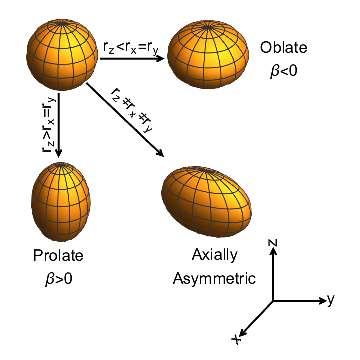
\includegraphics[scale=1]{Introduction_Figs/Deformation.png}
    \caption{Illustration of different kinds of deformation, where spherical symmetry is lost. Treating the vertical as the axis of symmetry, the prolate nucleus is contracted along this axis, but is still axially symmetric. The oblate nucleus is elongated along this axis, but otherwise axially symmetric. It is also possible for the nucleus to lose axial symmetry.}
    \label{fig:deformation}
\end{figure}